\section{Test cases for simple statecharts}
\label{testSimpeState}

In this section, we consider only statecharts that do not contain hierarchy and concurrency. Statecharts with hierarchy and concurrency will be explained afterwards.

%\todo[inline]{descrever aqui de forma intuitiva o que ser�o os test cases}

Each test case created will comprise:

\begin{itemize}

\item \textbf{A transition}. The transition that is being tested.

\item \textbf{An origin state}. The state from which the transition being tested is leaving from.

\item \textbf{A test path}. The path in the statechart used to activate the transition being tested.

\item \textbf{An expected state}. The state to which the transition being tested should redirect.

\end{itemize}

We start by making sure every reachable state in the statechart is covered. In order to do so, for each state $s$ in the statechart, we construct a path $p$ from the initial state to $s$. The path $p$ in said to be the \textit{coverage path of $s$}. All coverage paths generated are stored in a set called \textit{State Cover}, which is denoted by $C$. Therefore, $C$ is a set of sequence of transition labels, such that we can find an element from this set to reach any desired state starting from the initial one \cite{bogdanov}.

Since there is no hierarchy or concurrency in the statechart considered at this point, the construction of $C$ is similar to covering states of an automaton and it can be done through a depth search of the states. Find below a pseudocode for the method:

\begin{lstlisting}[caption={State Cover construction wrapper for simple statecharts}]
//Wrap method to contrusct the State Cover
//It receives as argument the initial state of a simple statechart
Set constructSetC(State initialState) {
	
	Set setC = new Set();

	Path emptyPath = "";

	List visited = new List();

	return constructSetCRec(initalState,emptyPath,setC,visited);
}
\end{lstlisting}


\begin{lstlisting}[caption={Recursive State Cover construction for simple statecharts}]
//Recursive function that will do all the work
//returns the State Cover set, or set C
Set constructSetCRec(State s, Path p, Set setC, List visited) {

	visited.add(s);

	setC.add(s,p);
	
	for (Transition t in s.getOutgGoingTransitions()) {
		
		State nextState = t.getDestiny();

		if (!visited.contains(nextState)) {

			Path nextCoveragePath = p + t.getLabel());

			constructSetCRec(nextState,nextCoveragePath,setC,visited);		
		}
	}
	
	return setC;
}

\end{lstlisting}

Now that we have the coverage for every reachable state, we need to trigger each transition on each state and create the test cases. For each transition there will be a test case, thus every transition in the diagram will be exercised at least once during testing.

Consider transition $t = (s,l,q)$, where $s$ is the original state, $l$ is the event label that triggers $t$ and $q$ is the incoming state. In the aforementioned algorithm, we computed that $s$ has coverage path $p$ such that $p \in C$ and $p$ is a sequence of labels. The test case $TC$ for transition $t$ ($t = (s,l,q)$) concatenates event labelled by $l$ to the end of $p$ that reaches state $q$. The process is repeated to all transitions in the statechart. The following algorithm describes the test cases creation:

\begin{lstlisting}[label={pseudocodeTestCase},caption{Test case creation for simple a simple statechart}]
//Function that prints the test cases for all transitions in a statechart
void generateTestCases(Statechart sc, Set setC) {

	for (State s in sc.getStates()) {
	
		Path coveragePath = setC.getCoveragePath(s);

		for (Transition t in s.getOutgGoingTransitions()) {

			print("Test case for "+t.getLabel());

			print("Origin state "+s.getName());

			Path testPath = coveragePath + t.getLabel();

			print("Test Path: "+testPath);

			State expectedState = t.getDestiny();

			print("Expected state: "+expectedState);
		}
	}
}
\end{lstlisting}


Consider the statechart in Figure \ref{fig:trocaPlano}, a model for purchase flow of a telco e-commerce. The model describes the flow for users changing their cellphone plan. They will be able to change plan if they are not employees from the telco company and are not committed to a loyalty contract. Additionally, they must perform the login so that the system is able to retrieve their information. This statechart models the requirement described in Subsection \ref{req1}.

\begin{figure}[htb]
\centering
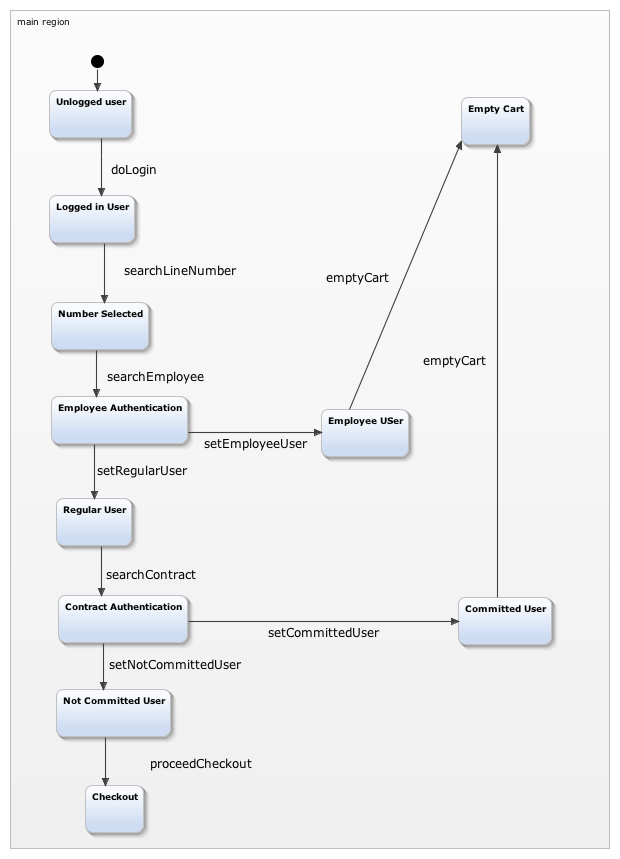
\includegraphics[width=10cm]{figuras/trocaPlano}
\caption{\label{fig:trocaPlano} A statechart for the plan change in a telco e-commerce}
\end{figure}

Since, hierarchy and orthogonality are not used in the presented  statechart (Figure \ref{fig:trocaPlano}), the technique presented above can be applied straight forward.

The construction of the \textit{State Cover} set, or $C$, is performed as follows:

\begin{enumerate}

\item We start at the initial state \textit{Unlogged User}. Since it is the initial state, its coverage path is the empty string, denoted by $e$.

\item Next, we recursively visit the states that can be reached from \textit{Unlogged User}. In our example, we get to state \textit{Logged in User}. In order to get to this state, it was necessary to go through transition $doLogin$. Therefore, the coverage path for \textit{Logged in User} is \textit{e doLogin}. Note that we concatenated the coverage path of the previous state to the undertaken transition.

\end{enumerate}

Once the construction of $C$ is concluded, we have the following coverage paths:

\begin{center}
\begin{tabular}{| l | p{10cm}|}

\hline

State & Coverage path \\ \hline

Unlogged user & e \\ \hline

Logged in User & e doLogin\\ \hline 

Number Selected & e doLogin searchLineNumber\\ \hline

Employee Authentication & e doLogin searchLineNumber searchEmployee\\ \hline

Employee User & e doLogin searchLineNumber searchEmployee setEmployeeUser \\ \hline

Empty Cart & e doLogin searchLineNumber searchEmployee setEmployeeUser emptyCart \\ \hline

Regular User & doLogin searchLineNumber searchEmployee setRegularUser \\ \hline

Contract Authentication & doLogin searchLineNumber searchEmployee setRegularUser searchContract \\ \hline

Committed User & doLogin searchLineNumber searchEmployee setRegularUser searchContract setCommittedUser \\ \hline

Not Committed User & doLogin searchLineNumber searchEmployee setRegularUser searchContract setNotCommittedUser \\ \hline

Checkout & doLogin searchLineNumber searchEmployee setRegularUser searchContract setNotCommittedUser proceedCheckout\\
\hline
\end{tabular}
\end{center}

Note that the empty string $e$ appears in the paths due to the unlabelled default transition entering the initial state \textit{Unlogged User}.

Then, we have to create a test case for every transition leaving each state. Let's take state \textit{Employee Authentication}, for example. It has two leaving transitions: $setEmployeeUser$ and $setRegularUser$. To guarantee they are exercised at least once during testing and that they go to their appropriate states, the following test cases are needed:

\begin{itemize}

\item Test case for \textit{\textbf{setEmployeeUser}}

Origin state: \textit{Employee Authentication}

Test Path: \textit{e doLogin searchLineNumber searchEmployee setEmployeeUser}

Expected state: \textit{Employee User}

\item Test case for \textit{\textbf{setRegularUser}}

Origin state: \textit{Employee Authentication}

Test Path: \textit{e doLogin searchLineNumber searchEmployee setRegularUser}

Expected state: \textit{Regular User}
\end{itemize}

Note that the \textit{test path} is the coverage path concatenated with the label of the tested transition. This procedure is similarly applied to all other transitions in the model.

